\documentclass[12pt, a4paper]{article}

\usepackage{lastpage}
\usepackage{mathtools}
\usepackage{xltxtra}
\usepackage{libertine}
\usepackage{amsmath}
\usepackage{amsthm}
\usepackage{amsfonts}
\usepackage{amssymb}
\usepackage{enumitem}
\usepackage{xcolor}
\usepackage[left=1.5cm, right=1.5cm, top=2cm, bottom=2cm, bindingoffset=0cm, headheight=15pt]{geometry}
\usepackage{fancyhdr}
\usepackage[russian]{babel}
% \usepackage[utf8]{inputenc}
\usepackage{catchfilebetweentags}
\usepackage{accents}
\usepackage{calc}
\usepackage{etoolbox}
\usepackage{mathrsfs}
\usepackage{wrapfig}

\providetoggle{useproofs}
\settoggle{useproofs}{false}

\pagestyle{fancy}
\lfoot{M3137y2019}
\rhead{\thepage\ из \pageref{LastPage}}

\newcommand{\R}{\mathbb{R}}
\newcommand{\Q}{\mathbb{Q}}
\newcommand{\C}{\mathbb{C}}
\newcommand{\Z}{\mathbb{Z}}
\newcommand{\B}{\mathbb{B}}
\newcommand{\N}{\mathbb{N}}

\newcommand{\const}{\text{const}}

\newcommand{\teormin}{\textcolor{red}{!}\ }

\DeclareMathOperator*{\xor}{\oplus}
\DeclareMathOperator*{\equ}{\sim}
\DeclareMathOperator{\Ln}{\text{Ln}}
\DeclareMathOperator{\sign}{\text{sign}}
\DeclareMathOperator{\Sym}{\text{Sym}}
\DeclareMathOperator{\Asym}{\text{Asym}}
% \DeclareMathOperator{\sh}{\text{sh}}
% \DeclareMathOperator{\tg}{\text{tg}}
% \DeclareMathOperator{\arctg}{\text{arctg}}
% \DeclareMathOperator{\ch}{\text{ch}}

\DeclarePairedDelimiter{\ceil}{\lceil}{\rceil}
\DeclarePairedDelimiter{\abs}{\left\lvert}{\right\rvert}

\setmainfont{Linux Libertine}

\theoremstyle{plain}
\newtheorem{axiom}{Аксиома}
\newtheorem{lemma}{Лемма}

\theoremstyle{remark}
\newtheorem*{remark}{Примечание}
\newtheorem*{exercise}{Упражнение}
\newtheorem*{consequence}{Следствие}
\newtheorem*{example}{Пример}
\newtheorem*{observation}{Наблюдение}

\theoremstyle{definition}
\newtheorem{theorem}{Теорема}
\newtheorem*{definition}{Определение}
\newtheorem*{obozn}{Обозначение}

\setlength{\parindent}{0pt}

\newcommand{\dbltilde}[1]{\accentset{\approx}{#1}}
\newcommand{\intt}{\int\!}

% magical thing that fixes paragraphs
\makeatletter
\patchcmd{\CatchFBT@Fin@l}{\endlinechar\m@ne}{}
  {}{\typeout{Unsuccessful patch!}}
\makeatother

\newcommand{\get}[2]{
    \ExecuteMetaData[#1]{#2}
}

\newcommand{\getproof}[2]{
    \iftoggle{useproofs}{\ExecuteMetaData[#1]{#2proof}}{}
}

\newcommand{\getwithproof}[2]{
    \get{#1}{#2}
    \getproof{#1}{#2}
}

\newcommand{\import}[3]{
    \subsection{#1}
    \getwithproof{#2}{#3}
}

\newcommand{\given}[1]{
    Дано выше. (\ref{#1}, стр. \pageref{#1})
}

\renewcommand{\ker}{\text{Ker }}
\newcommand{\im}{\text{Im }}
\newcommand{\grad}{\text{grad}}

\lhead{Математическая логика \textit{(практика)}}
\cfoot{}
\rfoot{18.2.2021}

\mathtoolsset{showonlyrefs=false}

\begin{document}

\begin{remark}
    Эти решения проверены только частично через \texttt{lean}, верность не гарантируется.
\end{remark}

\begin{exercise}[2.d]
    \(\vdash A \with B \to B \with A\)

    Докажем, что \(A \with B \vdash B \with A\), это эквивалентно искомому.
    \begin{align*}
        1.\quad & A \with B \tag{\(\in \Gamma\)}   \\
        2.\quad & A \with B \to A \tag{а. 4}       \\
        3.\quad & A \tag{M.P. 1, 2}                \\
        4.\quad & A \with B \to B \tag{а. 5}       \\
        5.\quad & B \tag{M.P. 1, 4}                \\
        6.\quad & A \to B \to A \with B \tag{a. 3} \\
        7.\quad & B \to A \with B \tag{M.P. 3,6}   \\
        8.\quad & A \with B \tag{M.P. 5,7}         \\
    \end{align*}
\end{exercise}

\begin{exercise}[2.e]
    \(\vdash A \to \neg \neg A\)

    Докажем, что \(A \vdash \neg \neg A\), это эквивалентно искомому.
    \begin{align*}
        1.\quad & A \tag{\(\in \Gamma\)}                                            \\
        2.\quad & A \to (\neg A \to A) \tag{a. 1}                                   \\
        3.\quad & \neg A \to A \tag{M.P. 1, 2}                                      \\
        4.\quad & \neg A \to \neg A \tag{доказано ранее}                            \\
        5.\quad & (\neg A \to \neg A) \to (\neg A \to A) \to \neg \neg A \tag{a. 9} \\
        6.\quad & (\neg A \to A) \to \neg \neg A \tag{M.P. 4,5}                     \\
        7.\quad & \neg \neg A \tag{M.P. 3,6}                                        \\
    \end{align*}
\end{exercise}

\begin{exercise}[2.f]
    \(A \with \neg A \vdash B\)

    \begin{align*}
        1.\quad  & A \with \neg A \tag{\(\in \Gamma\)}                               \\
        2.\quad  & A \with \neg A \to A \tag{а. 4}                                   \\
        3.\quad  & A \with \neg A \to \neg A \tag{а. 5}                              \\
        4.\quad  & A \tag{M.P. 1, 2}                                                 \\
        5.\quad  & \neg A \tag{M.P. 1, 3}                                            \\
        6.\quad  & A \to (\neg B \to A) \tag{a. 1}                                   \\
        7.\quad  & \neg B \to A \tag{M.P. 4, 6}                                      \\
        8.\quad  & \neg A \to (\neg B \to \neg A) \tag{a. 1}                         \\
        9.\quad  & \neg B \to \neg A \tag{M.P. 5, 8}                                 \\
        10.\quad & (\neg B \to A) \to (\neg B \to \neg A) \to \neg \neg B \tag{а. 9} \\
        11.\quad & (\neg B \to \neg A) \to \neg \neg B \tag{M.P. 7,10}               \\
        12.\quad & \neg \neg B \tag{M.P. 9,11}                                       \\
        13.\quad & \neg \neg B \to B \tag{a. 10}                                     \\
        14.\quad & B \tag{M.P. 12,13}                                                \\
    \end{align*}
\end{exercise}

\begin{exercise}[3.a]
    \(\neg A, B \vdash \neg(A \with B)\)

    \begin{align*}
        1.\quad & A \with B \to A \tag{a. 4}                                                   \\
        2.\quad & \neg A \to (A \with B) \to \neg A \tag{a. 1}                                 \\
        3.\quad & \neg A \tag{\(\in \Gamma\)}                                                  \\
        4.\quad & A \with B \to \neg A \tag{M.P. 2,3}                                          \\
        5.\quad & (A \with B \to A) \to (A \with B \to \neg A) \to \neg (A \with B) \tag{a. 9} \\
        6.\quad & (A \with B \to \neg A) \to \neg (A \with B) \tag{M.P. 1, 5}                  \\
        7.\quad & \neg (A \with B) \tag{M.P. 4,6}                                              \\
    \end{align*}
\end{exercise}

\begin{exercise}[3.b]
    \(A, \neg B \vdash \neg(A \with B)\)

    \begin{align*}
        1.\quad & A \with B \to B \tag{a. 4}                                                   \\
        2.\quad & \neg B \to (A \with B) \to \neg B \tag{a. 1}                                 \\
        3.\quad & \neg B \tag{\(\in \Gamma\)}                                                  \\
        4.\quad & A \with B \to \neg B \tag{M.P. 2,3}                                          \\
        5.\quad & (A \with B \to B) \to (A \with B \to \neg B) \to \neg (A \with B) \tag{a. 9} \\
        6.\quad & (A \with B \to \neg B) \to \neg (A \with B) \tag{M.P. 1, 5}                  \\
        7.\quad & \neg (A \with B) \tag{M.P. 4,6}                                              \\
    \end{align*}
\end{exercise}

\begin{exercise}[3.c]
    \(\neg A, \neg B \vdash \neg (A \with B)\)

    \begin{align*}
        1.\quad & A \with B \to B \tag{a. 4}                                                   \\
        2.\quad & \neg B \to (A \with B) \to \neg B \tag{a. 1}                                 \\
        3.\quad & \neg B \tag{\(\in \Gamma\)}                                                  \\
        4.\quad & A \with B \to \neg B \tag{M.P. 2,3}                                          \\
        5.\quad & (A \with B \to B) \to (A \with B \to \neg B) \to \neg (A \with B) \tag{a. 9} \\
        6.\quad & (A \with B \to \neg B) \to \neg (A \with B) \tag{M.P. 1, 5}                  \\
        7.\quad & \neg (A \with B) \tag{M.P. 4,6}                                              \\
    \end{align*}
\end{exercise}

\begin{exercise}[3.d]
    \(\neg A, \neg B \vdash \neg (A \lor B)\)

    \begin{align*}
        1.\quad  & (A \lor B \to A) \to (A \lor B \to \neg A) \to \neg (A \lor B) \tag{a. 9} \\
        2.\quad  & (A \to A) \to (B \to A) \to (A \lor B \to A) \tag{a. 8}                   \\
        3.\quad  & A \to A \tag{доказано раннее}                                             \\
        4.\quad  & (B \to A) \to (A \lor B \to A) \tag{M.P. 2,3}                             \\
        5.\quad  & \neg A \tag{\(\in\Gamma\)}                                                \\
        6.\quad  & \neg B \tag{\(\in\Gamma\)}                                                \\
        7.\quad  & \neg A \to \neg B \to B \to A \tag{3.g}                                   \\
        8.\quad  & \neg B \to B \to A \tag{M.P. 5, 7}                                        \\
        9.\quad  & B \to A \tag{M.P. 6, 8}                                                   \\
        10.\quad & A \lor B \to A \tag{M.P. 4, 9}                                            \\
        11.\quad & (A \lor B \to \neg A) \to \neg (A \lor B) \tag{M.P. 1, 10}                \\
        12.\quad & \neg A \to (A \lor B \to \neg A) \tag{a. 1}                               \\
        13.\quad & A \lor B \to \neg A \tag{M.P. 5,12}                                       \\
        14.\quad & \neg (A \lor B) \tag{M.P. 11,13}
    \end{align*}
\end{exercise}

\begin{exercise}[3.e]
    \(A, \neg B \vdash \neg (A \to B)\)

    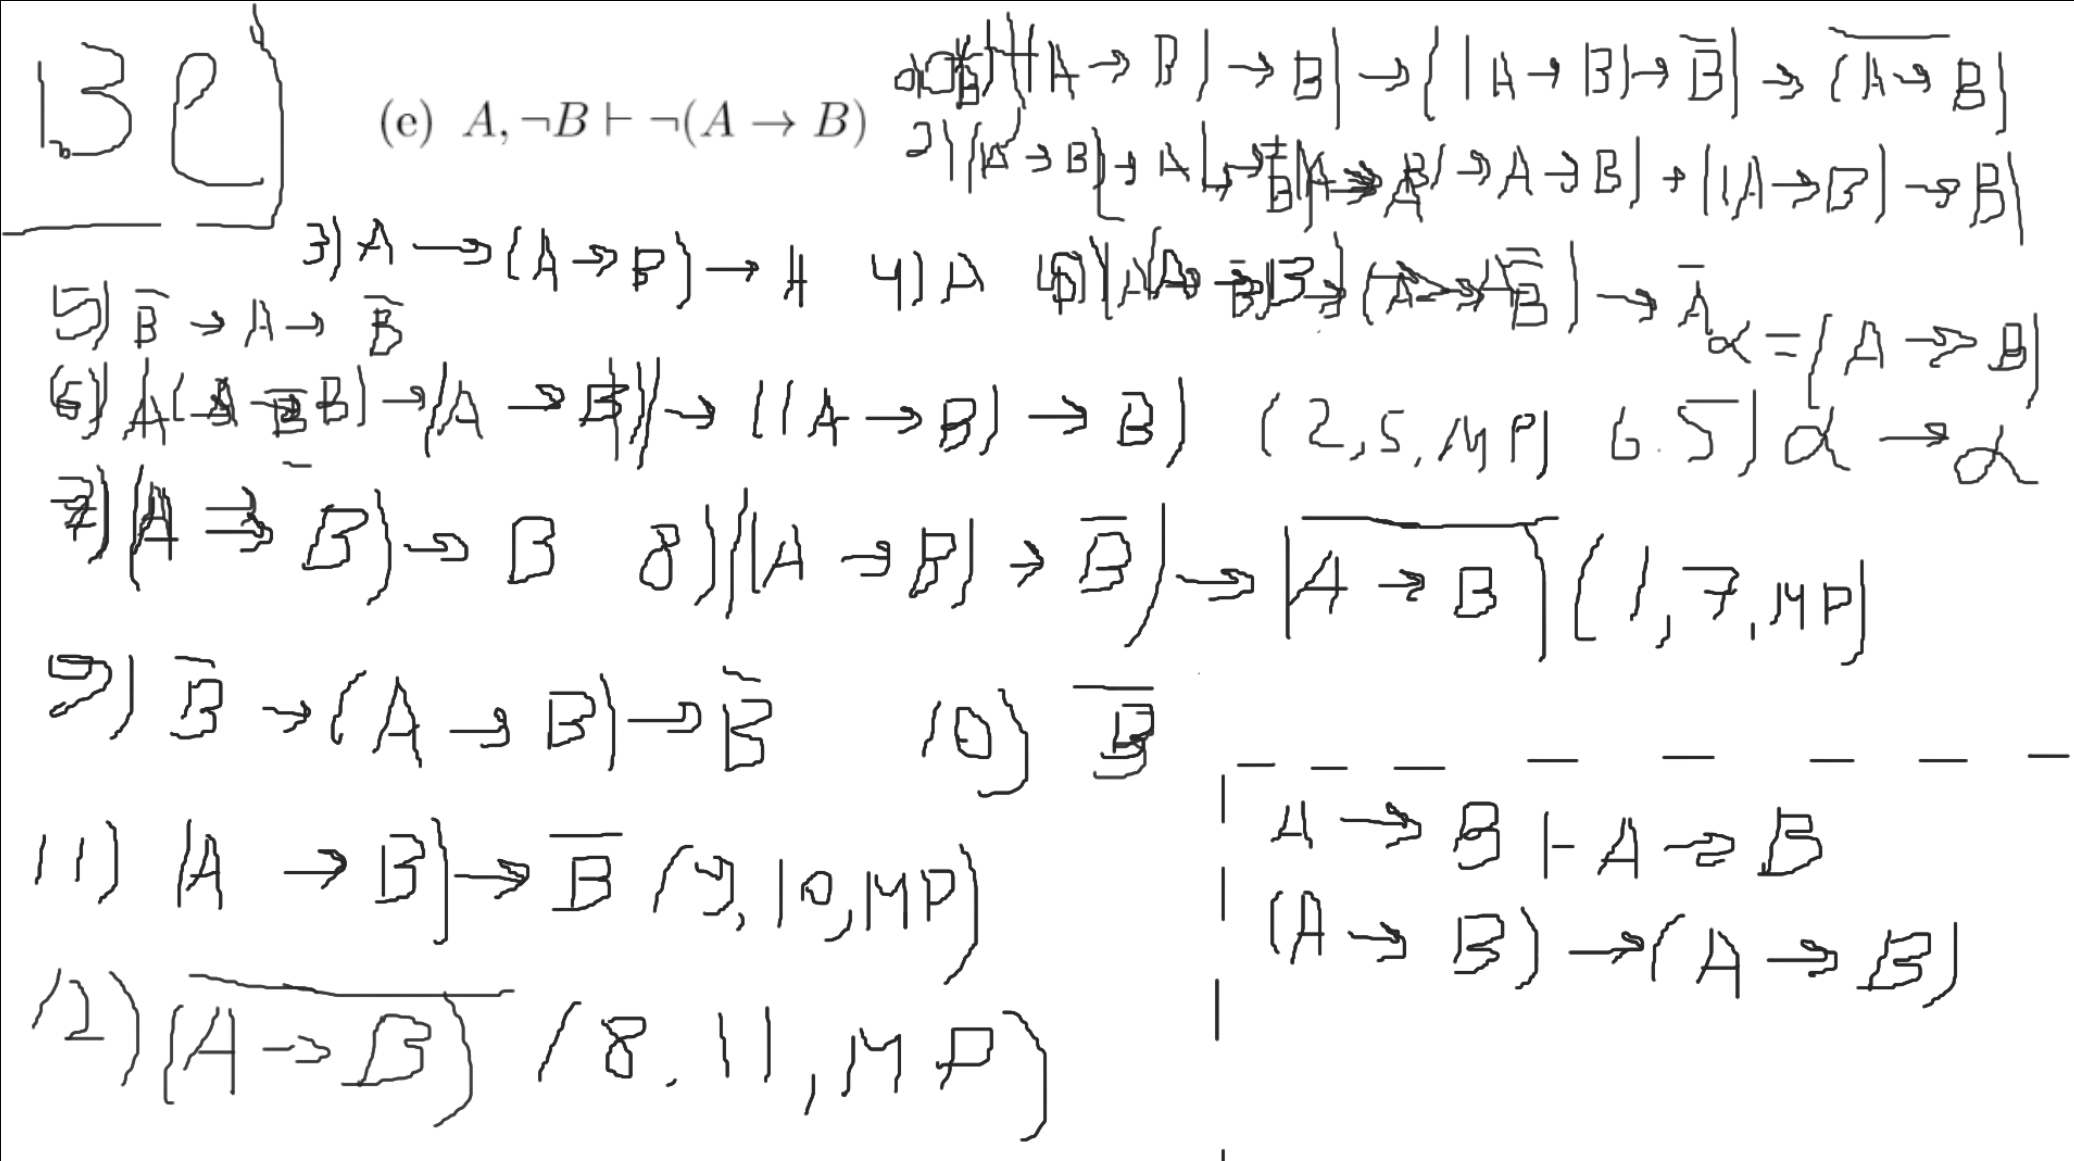
\includegraphics[width=\textwidth]{images/1.3.e.png}
\end{exercise}

\begin{exercise}[3.f]
    \(\neg A, B \vdash A \to B\)

    Докажем \(\neg A, B, A \vdash B\), т.к. это эквивалентно по теореме об индукции.

    \begin{align*}
        1.\quad & B \tag{\(\in \Gamma\)} \\
    \end{align*}
\end{exercise}

\begin{exercise}[3.g]
    \(\neg A, \neg B \vdash A \to B\)

    Докажем \(\neg A, \neg B, A \vdash B\), т.к. это эквивалентно по теореме об индукции.

    \begin{align*}
        1.\quad  & A \tag{\(\in \Gamma\)}                                            \\
        2.\quad  & \neg A \tag{\(\in \Gamma\)}                                       \\
        3.\quad  & A \to (\neg B \to A) \tag{a. 1}                                   \\
        4.\quad  & \neg B \to A \tag{M.P. 1, 3}                                      \\
        5.\quad  & \neg A \to (\neg B \to \neg A) \tag{a. 1}                         \\
        6.\quad  & \neg B \to \neg A \tag{M.P. 2, 5}                                 \\
        7.\quad  & (\neg B \to A) \to (\neg B \to \neg A) \to \neg \neg B \tag{а. 9} \\
        8.\quad  & (\neg B \to \neg A) \to \neg \neg B \tag{M.P. 4, 7}               \\
        9.\quad  & \neg \neg B \tag{M.P. 6, 8}                                       \\
        10.\quad & \neg \neg B \to B \tag{a. 10}                                     \\
        11.\quad & B \tag{M.P. 9, 10}                                                \\
    \end{align*}
\end{exercise}

\begin{exercise}[3.h]
    \(\vdash (A \to B) \to (B \to C) \to (A \to C)\)

    \begin{align*}
                                & \vdash (A \to B) \to (B \to C) \to (A \to C) \\
        (A \to B)               & \vdash (B \to C) \to (A \to C)               \\
        (A \to B), (B \to C)    & \vdash (A \to C)                             \\
        (A \to B), (B \to C), A & \vdash C
    \end{align*}
    \begin{align*}
        1.\quad & A \tag{\(\in \Gamma\)}       \\
        2.\quad & A \to B \tag{\(\in \Gamma\)} \\
        3.\quad & B \tag{M.P. 1,2}             \\
        4.\quad & B \to C \tag{\(\in\Gamma\)}  \\
        5.\quad & C \tag{M.P. 3,4}             \\
    \end{align*}
\end{exercise}

\begin{exercise}[3.i]
    \(\vdash (A \to B) \to (B \to C) \to (C \to A)\)

    Это утверждение не тавтология, что проверяется подстановкой \(0,0,1\). В силу корректности исчисления высказываний из пустого множества можно вывести только тавтологии, таким образом это утверждение не выводится.
\end{exercise}

\begin{exercise}[3.j]
    \(\vdash (A \to B) \to (\neg B \to \neg A)\)

    \begin{align*}
                          & \vdash (A \to B) \to (\neg B \to \neg A) \\
        (A \to B)         & \vdash \neg B \to \neg A                 \\
        (A \to B), \neg B & \vdash \neg A
    \end{align*}
    \begin{align*}
        1.\quad & A \to B \tag{\(\in\Gamma\)}                        \\
        2.\quad & \neg B \tag{\(\in\Gamma\)}                         \\
        3.\quad & \neg B \to A \to \neg B \tag{a. 1}                 \\
        4.\quad & A \to \neg B \tag{M.P. 2,3}                        \\
        5.\quad & (A \to B) \to (A \to \neg B) \to \neg A \tag{a. 9} \\
        6.\quad & (A \to \neg B) \to \neg A \tag{M.P. 1,5}           \\
        7.\quad & \neg A \tag{M.P. 4,6}                              \\
    \end{align*}
\end{exercise}

\begin{exercise}[4.a]
    \(\vdash A \lor \neg A\)

    \begin{align*}
        1.\quad & A \to A \lor \neg A \tag{aкс. 6}                                                                                      \\
        2.\quad & \neg A \to A \lor \neg A \tag{aкс. 7}                                                                                 \\
        3.\quad & \neg \neg (A \lor \neg A) \to \neg A \tag{закон контрапозиции}                                                        \\
        4.\quad & \neg (A \lor \neg A) \to \neg \neg A \tag{закон контрапозиции}                                                        \\
        5.\quad & (\neg (A\lor \neg A) \to \neg A) \to (\neg (A \lor \neg A) \to \neg \neg A) \to \neg \neg (A\lor \neg A) \tag{акс. 9} \\
        6.\quad & (\neg (A \lor \neg A) \to \neg \neg A) \to \neg \neg (A\lor \neg A) \tag{M.P. 4,6}                                    \\
        7.\quad & \neg \neg (A\lor \neg A) \tag{M.P. 5,7}                                                                               \\
        8.\quad & \neg \neg (A \lor \neg A) \to A \lor \neg A \tag{акс. 10}                                                             \\
        9.\quad & A \lor \neg A \tag{M.P. 8,9}                                                                                          \\
    \end{align*}
\end{exercise}

\begin{exercise}[4.b]
    \(\vdash A \with B \to \neg (\neg A \lor \neg B)\)

    \begin{align*}
        1.\quad  & A\&B \vdash \neg (\neg A  \lor \neg B) \tag{т. о дедукции}                                                    \\
        2.\quad  & (\neg A  \lor \neg B \to A) \to (\neg A  \lor \neg B  \to \neg A) \to  \neg (\neg A  \lor \neg B) \tag{акс.9} \\
        3.\quad  & A\&B \to A \tag{акс. 4}                                                                                       \\
        4.\quad  & A\&B \to B \tag{акс. 5}                                                                                       \\
        5.\quad  & A \tag{M.P. 3, 1}                                                                                             \\
        6.\quad  & B \tag{M.P. 4, 1}                                                                                             \\
        7.\quad  & A \to (\neg A  \lor \neg B) \to A \tag{акс.1}                                                                 \\
        8.\quad  & (\neg A  \lor \neg B) \to A \tag{M.P. 7, 5}                                                                   \\
        9.\quad  & (\neg A  \lor \neg B  \to \neg A) \to  \neg (\neg A  \lor \neg B) \tag{M.P. 2, 8}                             \\
        10.\quad & (\neg A \to \neg A) \to (\neg B \to \neg A) \to (\neg A  \lor \neg B \to \neg A) \tag{акс. 8}                 \\
        11.\quad & (\neg B \to \neg A) \to (\neg A  \lor \neg B \to \neg A) \tag{M.P. 8 и известный факт}                        \\
        12.\quad & B, A \vdash \neg B \to \neg A \text{ равносильно } B, A, \neg B \vdash \neg A \tag{т. о дедукции}             \\
        13.\quad & (A \to B) \to (A \to \neg B) \to \neg A \tag{акс.9}                                                           \\
        14.\quad & \neg A \tag{дважды аксиома 1 из \(B\) и \(\neg B\)}                                                           \\
        15.\quad & \neg B \to \neg A \tag{доказали по дедукции}                                                                  \\
        16.\quad & (\neg A  \lor \neg B \to \neg A) \tag{M.P. 11, 15}                                                            \\
        17.\quad & \neg (\neg A  \lor \neg B) \tag{M.P. 9, 16}
    \end{align*}

\end{exercise}

\begin{exercise}[4.c]
    \(\vdash \neg (\neg A \with \neg B) \to A \lor B\)
\end{exercise}

\begin{exercise}[4.d]
    \(\vdash A \with \neg A \to A \lor B\)

    \begin{align*}
                       & \vdash A \with \neg A \to A \lor B \\
        A \with \neg A & \vdash A \lor B
    \end{align*}
    \begin{align*}
        1.\quad & A \with \neg A \tag{\(\in\Gamma\)} \\
        2.\quad & A \with \neg A \to A \tag{a. 4}    \\
        3.\quad & A \tag{M.P. 1,2}                   \\
        4.\quad & A \to A \lor B \tag{a. 6}          \\
        5.\quad & A \lor B \tag{M.P. 3,4}            \\
    \end{align*}
\end{exercise}

\begin{exercise}[4.e]
    \(\vdash ((A \to B) \to A) \to A\)

    Идея решения --- рассмотрим три случая : \(A \in \Gamma; \neg A, B \in \Gamma; \neg A, \neg B \in \Gamma\)
\end{exercise}

\begin{exercise}[5]
    Даны высказывания $\alpha$ и $\beta$, причём $\vdash \alpha\rightarrow\beta$ и $\alpha\not\equiv\beta$.
    Укажите способ построения высказывания $\gamma$, такого, что
    $\vdash\alpha\rightarrow\gamma$ и $\vdash\gamma\rightarrow\beta$, причём $\alpha\not\equiv\gamma$ и
    $\beta\not\equiv\gamma$.

    Решение, рассказанное на паре \(\gamma : = \alpha \with \beta\), неверное, т.к. при тавтологии \(\beta\) выполняется \(\alpha \equiv \gamma\).

    Верное решение: пусть множество подстановок, на которых \(\alpha\) выполняется --- \(\mathcal{A}\), для \(\beta\) --- \(\mathcal{B}\). Несложно заметить, что \(\mathcal{A}\subset \mathcal{B}\), при этом \(|\mathcal{A}| < |\mathcal{B}|\). Если \(|\mathcal{A}| < |\mathcal{B}| - 1\), то можно найти множество между ними, т.е. \(\mathcal{A}\subset \mathcal{C}\subset \mathcal{B}\). Если \(|\mathcal{A}| = |\mathcal{B}| - 1\), то нужно ввести новую переменную, чтобы разница стала больше.
\end{exercise}

\begin{exercise}[6]
    \(\alpha \vdash \beta, \neg \alpha \vdash \beta \Rightarrow\ \vdash \beta\)

    \begin{align*}
        1.\quad  & \alpha \tag{\(\in\Gamma\)}                                                              \\
        2.\quad  & \alpha \to (\neg \beta \to \alpha) \tag{a. 1}                                           \\
        3.\quad  & \neg \beta \to \alpha \tag{M.P. 1,2}                                                    \\
        4.\quad  & \neg \alpha \tag{\(\in\Gamma\)}                                                         \\
        5.\quad  & \neg \alpha \to (\neg \beta \to \neg \alpha) \tag{a. 1}                                 \\
        6.\quad  & \neg \beta \to \neg \alpha \tag{M.P. 4,5}                                               \\
        7.\quad  & (\neg \beta \to \alpha) \to (\neg \beta \to \neg \alpha) \to \neg \neg \beta \tag{a. 9} \\
        8.\quad  & (\neg \beta \to \neg \alpha) \to \neg \neg \beta \tag{M.P. 3,7}                         \\
        9.\quad  & \neg \neg \beta \tag{M.P. 6,8}                                                          \\
        10.\quad & \neg \neg \beta \to \beta \tag{a. 10}                                                   \\
        11.\quad & \beta \tag{M.P. 9,10}                                                                   \\
    \end{align*}
\end{exercise}

\end{document}